\documentclass[10pt, aspectratio=169]{beamer}

% Modern, clean theme
\usetheme{Boadilla} % Uses standard Boadilla theme
\definecolor{primary}{RGB}{43, 61, 79}
\definecolor{accent}{RGB}{204, 85, 0}
\definecolor{highlight}{RGB}{46, 134, 171}
\setbeamercolor{frametitle}{bg=primary, fg=white}
\setbeamercolor{palette primary}{bg=primary, fg=white}
\setbeamercolor{progress bar}{fg=accent, bg=gray!30}
\setbeamercolor{alerted text}{fg=accent}
\setbeamercolor{block title}{bg=primary!80, fg=white}
\setbeamercolor{block body}{bg=primary!10, fg=black}
\setbeamercolor{block title example}{bg=highlight, fg=white}
\setbeamercolor{block body example}{bg=highlight!10, fg=black}

\usepackage{amsmath, amssymb, amsfonts}
\usepackage{graphicx}
\graphicspath{{../figures/}{../../figures/}{./figures/}}
\usepackage{tikz}
\usepackage{booktabs}
\usepackage{algorithm}
\usepackage{algpseudocode}

% Math shortcuts
\newcommand{\R}{\mathbb{R}}
\newcommand{\E}{\mathbb{E}}
\newcommand{\Prob}{\mathbb{P}}
\DeclareMathOperator{\Var}{Var}
\DeclareMathOperator{\Cov}{Cov}
\DeclareMathOperator{\sgn}{sign}
\DeclareMathOperator*{\argmin}{arg\,min}
\newcommand{\Ind}[1]{\mathbb{I}\{#1\}}
\newcommand{\given}{\mid}
\newcommand{\cX}{\mathcal{X}}
\newcommand{\cY}{\mathcal{Y}}
\newcommand{\cS}{\mathcal{S}}
\newcommand{\cR}{\mathcal{R}}

\title{The Case for Voluntary Disclosure}
\subtitle{Strategic Feature Revelation in Regression and Classification}
\author{Author 1 \and Author 2}
\institute{Google DeepMind}
\date{\today}

\begin{document}

\maketitle

\begin{frame}{Outline}
  \setbeamertemplate{section in toc}[sections numbered]
  \tableofcontents[hideallsubsections]
\end{frame}

\section{Introduction and Motivation}

\begin{frame}{Motivation: Financial Firm Valuation}
  \begin{block}{The Core Question}
    Should a predictive model enforce \textbf{mandatory} feature disclosure or allow \textbf{voluntary} disclosure by participants?
  \end{block}
  \vspace{0.3cm}
  \begin{itemize}
      \item \textbf{Scenario:} Market estimating a firm's valuation.
      \item \textbf{Issue:} Firms strategically reveal features. Some seek overvaluation (to raise stock prices), while others prefer undervaluation (e.g., for stock buybacks).
      \item \textbf{Intuition:} If a firm's preference aligns with the market objective, selective disclosure filters out noisy signals. If misaligned, it distorts information.
  \end{itemize}
\end{frame}

\section{Problem Formulation}

\begin{frame}{Sender-Receiver Game Model}
    \begin{columns}[T]
    \column{0.5\textwidth}
    \textbf{The Setting:}
    \begin{itemize}
        \item State drawn by Nature: $x$ (features), $y$ (ground truth), $u$ (sender's preferred value).
        \item \textbf{Sender} observes $(u, x)$ and chooses action $A \in \{\emptyset, x\}$ (withhold or disclose).
        \item \textbf{Noisy Channel:} Message $M$ is received. If Sender discloses $x$, Receiver gets it with probability $1-q$, and gets $\emptyset$ with probability $q$.
    \end{itemize}

    \column{0.5\textwidth}
    \textbf{The Game:}
    \begin{itemize}
        \item \textbf{Receiver} commits to strategy $\hat{y}(M)$.
        \item \textbf{Sender} perfectly best-responds by minimizing their expected loss $\ell(u, \hat{y}(M))$.
        \item \textbf{Stackelberg Equilibrium:} Receiver optimizes $\hat{y}$ anticipating Sender's rational reaction.
    \end{itemize}
    \end{columns}
\end{frame}

\begin{frame}{Mandatory vs. Voluntary Regimes}
    \begin{block}{Mandatory Disclosure (Vanilla Risk)}
      Sender is forced to reveal $A = x$.
      Vanilla Risk: $R_V := \E[\ell(Y, \hat{y}_V(M))]$
    \end{block}

    \begin{block}{Voluntary Disclosure (Strategic Risk)}
      Sender is allowed to withhold features opportunistically.
      Strategic Risk: $R_S := \min_{\hat{y}} \E[\ell(Y, \hat{y}(M))]$
    \end{block}
    
    \vspace{0.2cm}
    \begin{alertblock}{Strategic Advantage}
      A \textbf{strategic advantage} exists if permitting voluntary disclosure yields a strictly lower expected loss for the Receiver: \quad $R_S < R_V$.
    \end{alertblock}
\end{frame}

\section{Strategic Advantage in Regression}

\begin{frame}{Regression: Problem Setup}
    \begin{itemize}
        \item \textbf{Outcome Space:} $\cY = \R$.
        \item \textbf{Loss Function:} Mean Squared Error $\ell(y, \hat{y}) = (y - \hat{y})^2$.
        \item All random variables $(U, X, Y)$ are zero-mean.
    \end{itemize}
    \vspace{0.3cm}
    \begin{exampleblock}{Vanilla Risk (Mandatory Disclosure)}
      For a linear strategy parameterized by $b$ (i.e., $\hat{y}_V(x) = b^\top x$ and $\hat{y}(\emptyset) = 0$), the optimal vanilla risk is achieved at $b_Y = \Var(X)^{-1}\Cov(X,Y)$:
      \begin{equation*}
          R_V^\star(q) = \Var(Y) - (1-q) \Var(b_Y^\top X)
      \end{equation*}
    \end{exampleblock}
\end{frame}

\begin{frame}{Regression: Voluntary Disclosure Dynamics}
    Let the Receiver's linear strategy be parameterized by $b$.
    
    We define two critical scalar fields:
    \begin{align*}
        F(x,u) &:= (2u - b^\top x) b^\top x \quad \text{(Sender's decision rule)}\\
        G(x,y) &:= (2y - b^\top x) b^\top x \quad \text{(Receiver's relative gain)}
    \end{align*}
    
    \begin{block}{Sender's Best Response}
        The Sender discloses the feature $A(x,u)=x \iff F(x,u) > 0$.
    \end{block}
    
    \textbf{Strategic Risk Formulation:}
    \begin{equation*}
        R_S(b, q) = \Var(Y) - (1-q)\E\big[G(X,Y)\Ind{F(X,U) > 0}\big]
    \end{equation*}
\end{frame}

\begin{frame}{Regression: The Advantage Conditions}
    \begin{theorem}[Sufficiency Condition]
      A strategic advantage ($R_S^\star(q) < R_V^\star(q)$) exists if there exists $b \in \R^d$ such that:
      \begin{equation*}
        \|U{-}Y\|_2 < \frac{\E\big[| G(X,Y)|\big] - \Var(b_Y^\top X)}{4\sqrt{\Var(b_Y^\top X)}} - \frac{\Var((b{-}b_Y)^\top X)}{4\sqrt{\Var(b_Y^\top X)}}
      \end{equation*}
    \end{theorem}
    \vspace{0.2cm}
    \begin{theorem}[Necessary Condition]
      A necessary condition for a strategic advantage to exist is:
      \begin{equation*}
        \max_b \Big( \E\big[| G(X,Y)|\big] - \Var(b_Y^\top X) - \Var((b{-}b_Y)^\top X) \Big) > 0
      \end{equation*}
    \end{theorem}
    \alert{Insight:} Both bounds are independent of channel noise $q$. Noise scales the magnitude but not the existence of the advantage.
\end{frame}

\begin{frame}{Regression: Heatmap Verification}
    \begin{columns}
        \column{0.5\textwidth}
        \begin{itemize}
            \item Simulation over a zero-mean Gaussian family for $(X,Y,U)$.
            \item $\Cov(X,Y) = \Cov(X,U) = 0.2$.
            \item Channel noise probability $q$ swept along $y$-axis.
            \item Preference alignment $\Cov(Y,U)$ swept along $x$-axis.
            \item The dotted black line delineates theoretical "If and Only If" bounds!
        \end{itemize}
        \column{0.5\textwidth}
        \begin{figure}
            \centering
            
\includegraphics[height=0.7\textheight,width=\textwidth,keepaspectratio]{regression_strategic_advantage.png}
        \end{figure}
    \end{columns}
\end{frame}

\section{Strategic Advantage in Classification}

\begin{frame}{Classification: Setup and Voluntary Responses}
    \begin{itemize}
        \item \textbf{Outcome Space:} $\cY = \{-1,+1\}$ (Discrete Labels).
        \item \textbf{Loss Function:} $0-1$ Loss $\ell(y, \hat{y}) = \Ind{\hat{y} \neq y}$.
        \item \textbf{Vanilla Risk:} $R_V^\star(q) = q\Prob(Y=-\sgn(\E[Y])) + (1-q)\E\Big[\frac{1-|\eta(X)|}{2}\Big]$
    \end{itemize}

    \begin{block}{The Default Option Dynamics}
        Receiver commits to a \textbf{default prediction} $\hat{y}(\emptyset) = i \in \{-1, +1\}$.
        \begin{itemize}
            \item Sender with preference $u$ withholds if $u = i$.
            \item Sender discloses if $u = -i$ to try shifting the prediction.
            \item Observing $X$ thus reveals $U = -i$, prompting Receiver optimal posterior $\sgn(\E[Y|X=x, U=-i])$.
        \end{itemize}
    \end{block}
\end{frame}

\begin{frame}{Classification: Equilibrium and Advantage}
    Because there are only two default options, the Stackelberg Equilibrium simply chooses the default $\cS_1$ or $\cS_{-1}$ achieving minimal Strategic Risk.
    
    \begin{theorem}[Stackelberg Equilibrium]
    \begin{itemize}
        \item For $q=1$, strategy aligned with prior mean is strictly better.
        \item For lower $q$'s, depending on distributions, an intermediate threshold $q^\star \in [0,1]$ exists governing when the optimal default strategy switches.
    \end{itemize}
    Unlike regression, channel noise $q$ governs BOTH the \textbf{magnitude} and \textbf{direction} of strategic advantage in specific distribution cases.
    \end{theorem}
\end{frame}

\begin{frame}{Classification: Heatmap Verification}
    \begin{columns}
        \column{0.45\textwidth}
        \begin{itemize}
            \item Discrete labels $(Y,U) \in \{-1,1\}^2$.
            \item Varying discrete preference alignment $\Cov(Y,U)$ on $x$-axis.
            \item Features from Gaussian Mixture Model $X|Y,U$.
            \item The theoretical boundary (dotted black) perfectly predicts advantage zones.
        \end{itemize}
        \column{0.55\textwidth}
        \begin{figure}
            \centering
            
\includegraphics[height=0.7\textheight,width=\textwidth,keepaspectratio]{classification_strategic_advantage.png}
        \end{figure}
    \end{columns}
\end{frame}

\section{The Learning Problem}

\begin{frame}{Learning in Unknown Environments}
    So far, we assumed the joint distribution $(X,U,Y)$ was completely known.
    We now expand to:
    
    \begin{enumerate}
        \item \textbf{Static Learning:} Receiver estimates parameters and risks offline from a bounded population sample $\mathcal{D} = \{(x_i, u_i, y_i)\}_{i=1}^n$.
        \item \textbf{Dynamic Learning:} Receiver learns parameters online across repeated interactions using Explore-Then-Commit strategies.
    \end{enumerate}
\end{frame}

\begin{frame}{Static Learning: Generalization Bounds}
    Receiver computes empirical Vanilla Risk $\hat{R}_V$ and empirical Strategic Risk $\hat{R}_S$.
    
    \begin{theorem}[Finite-Sample Generalization]
        With probability $1-\delta$, estimation errors scale as $\mathcal{O}\left(\frac{1}{\sqrt{n}}\right)$:
        \begin{align*}
            |\hat{R}_V(q) - R_V(q)| &\le \mathcal{O}\left( \dots \sqrt{\frac{d + \log(1/\delta)}{n}} \right) \\
            |\hat{R}_S(\hat{b}^\star,q) - R_S^\star(q)| &\le \mathcal{O}\left( \dots \sqrt{\frac{d + \log(1/\delta)}{n}} \right)
        \end{align*}
        Thus, the empirical regret gap reliably proxies the true Stackelberg equilibrium as $n \to \infty$.
    \end{theorem}
\end{frame}

\begin{frame}{Static Learning Empirical Convergence}
    \begin{columns}
        \column{0.4\textwidth}
        \textbf{Convergence Rate Simulation}
        \vspace{0.3cm}
        \begin{itemize}
            \item Expected gap error $|(\hat{R}_S - \hat{R}_V) - \Delta R^\star|$ shrinks linearly when plotted against $1/\sqrt{n}$.
            \item Confirms the $\mathcal{O}(1/\sqrt{n})$ theoretical reduction rate.
        \end{itemize}
        \column{0.6\textwidth}
        \begin{figure}
            \centering
            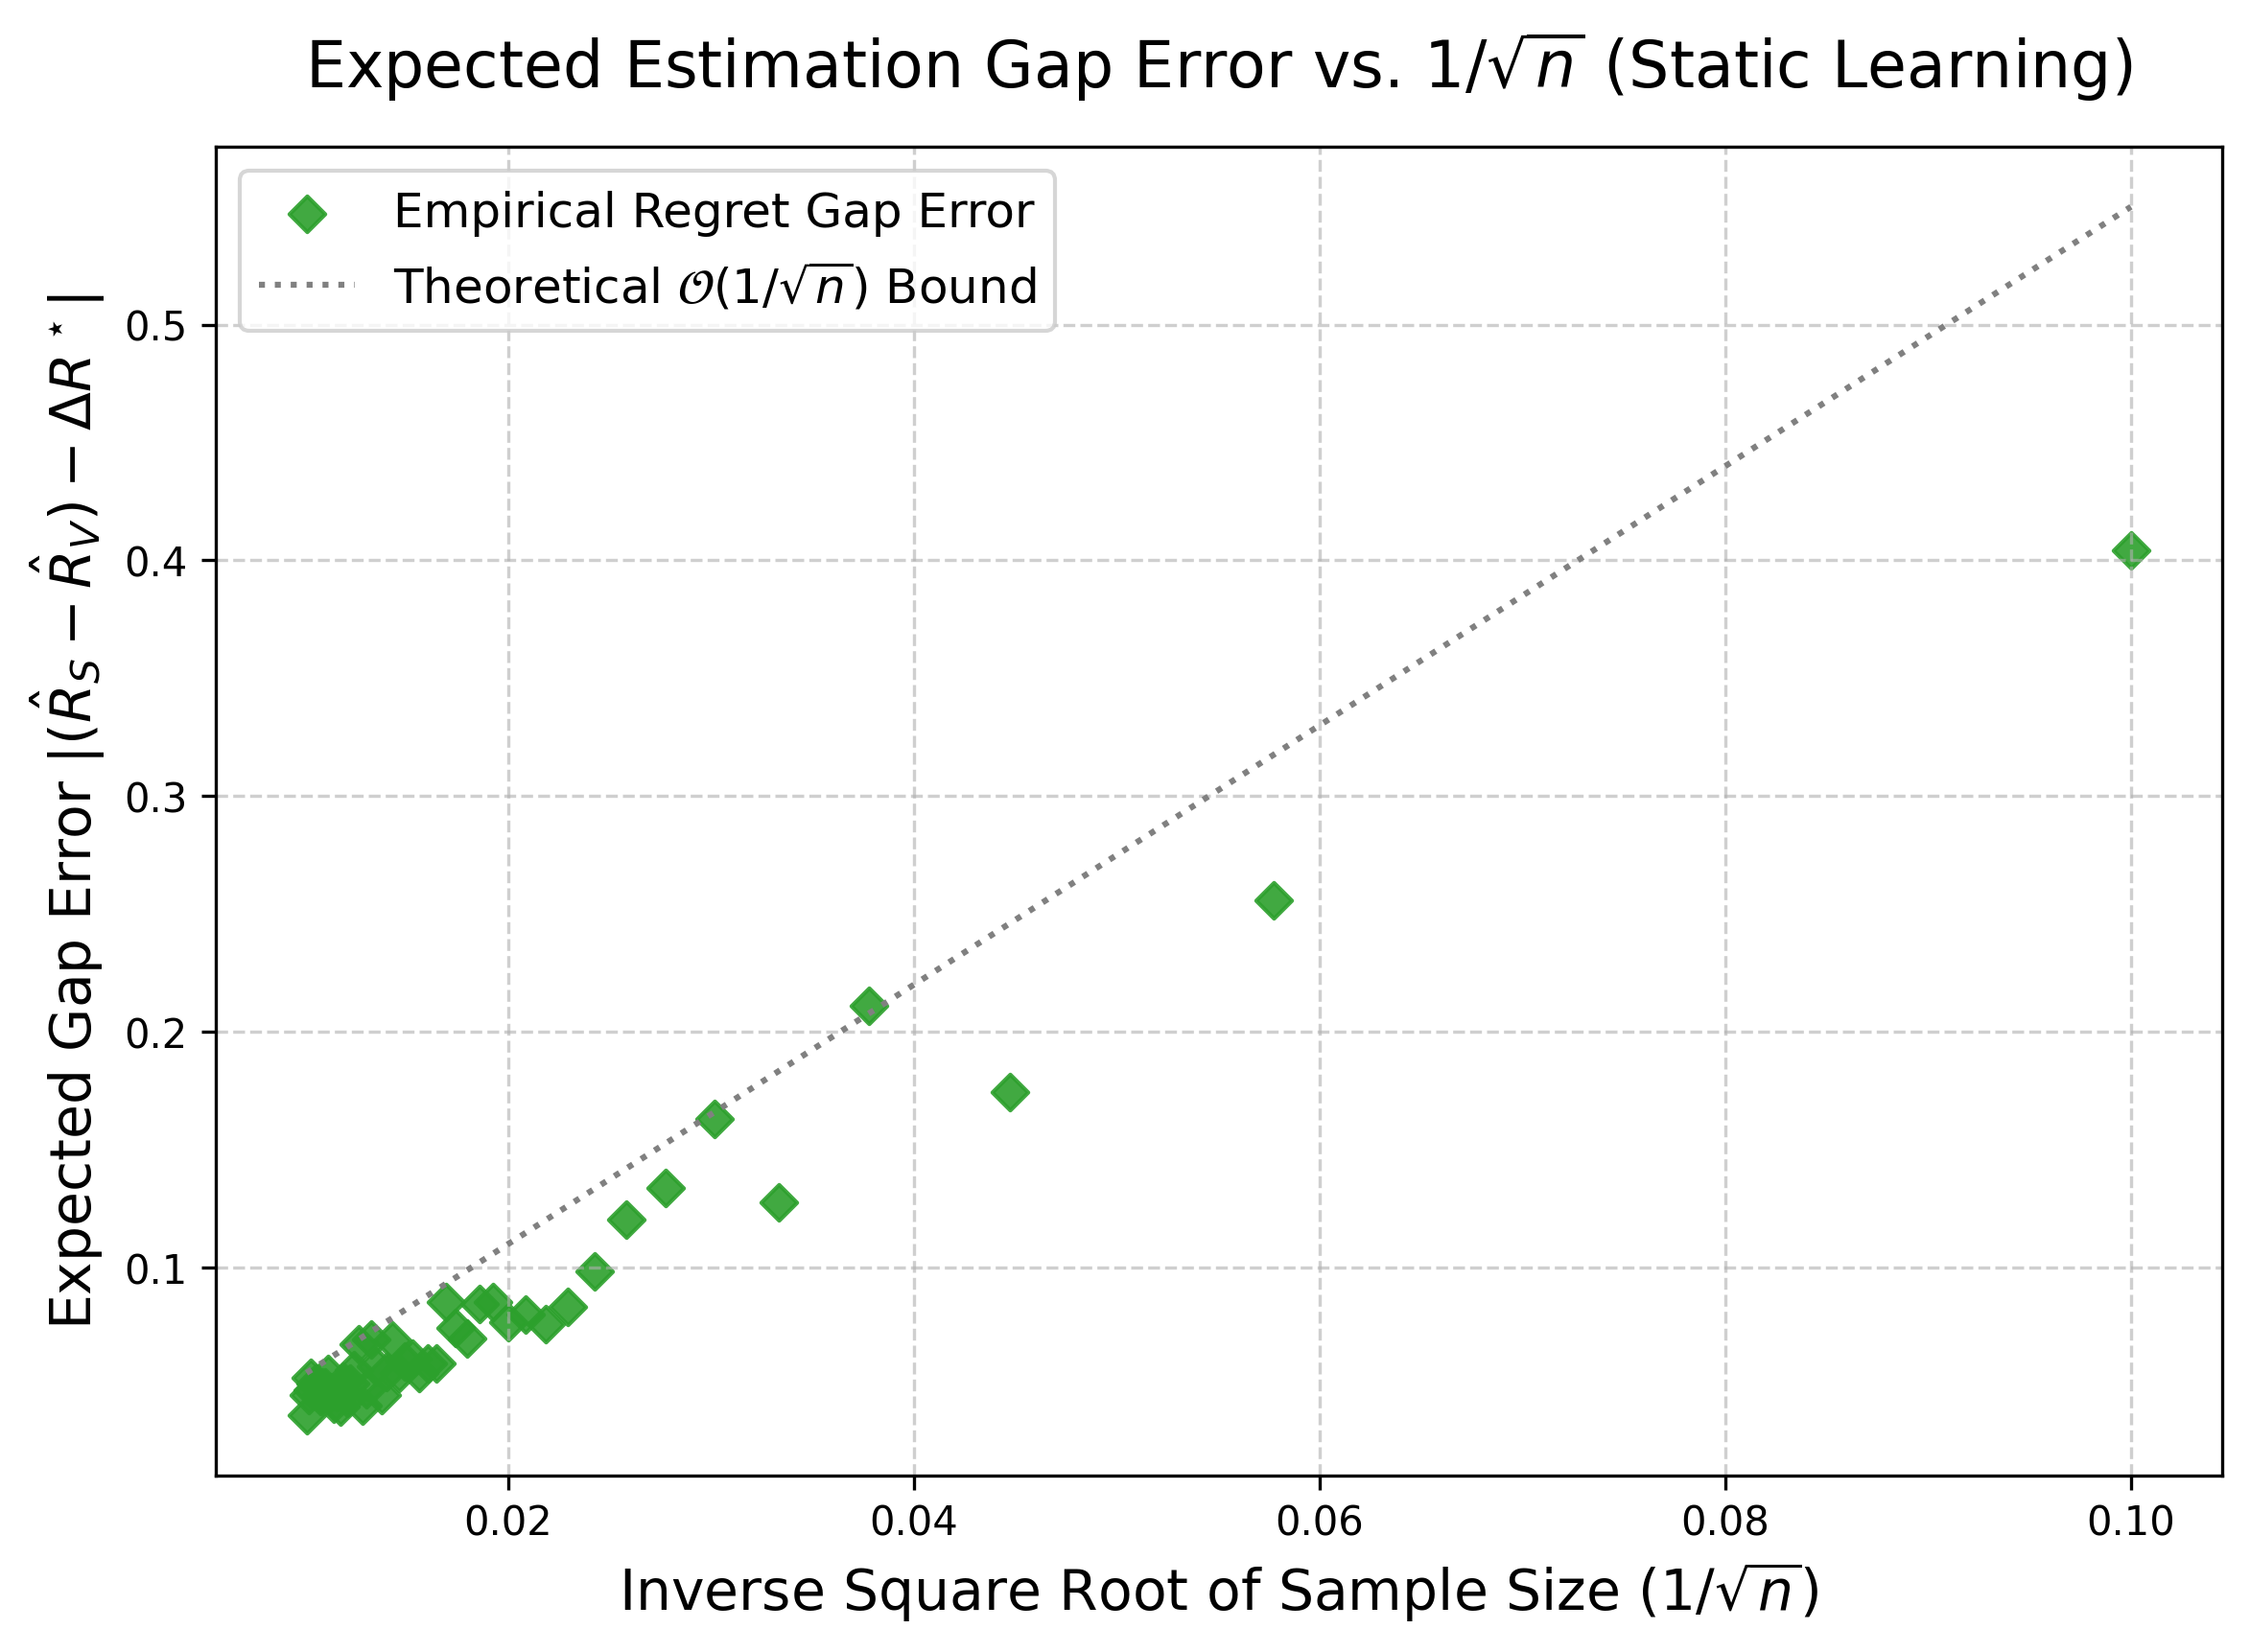
\includegraphics[height=0.7\textheight,width=\textwidth,keepaspectratio]{static_learning_gap_error.png}
        \end{figure}
    \end{columns}
\end{frame}

\begin{frame}{Dynamic Learning}
    Receiver minimizes cumulative regret over $T$ sequential interactions:
    \begin{equation*}
        \mathcal{R}_T = \sum_{t=1}^T \ell\big(y_t, \hat{y}_t(M_t)\big) - T \cdot \min \{ R_V^\star, R_S^\star \}
    \end{equation*}

    \begin{block}{Explore-Then-Commit (ETC) Algorithm}
        \begin{enumerate}
            \item \textbf{Explore:} For $t=1 \dots N$, enforce Voluntary regime. Observe data and maintain running empirical estimates $\hat{R}_V, \hat{R}_S$.
            \item \textbf{Switch:} At $N+1$, permanently commit to whichever regime (Voluntary or Mandatory) had lower estimated risk.
            \item \textbf{Commit:} Continually refine the predictor weights online under the designated regime for the remainder of time $T$.
        \end{enumerate}
    \end{block}
\end{frame}

\begin{frame}{Dynamic Learning Regret Analysis}
    \begin{theorem}
        The ETC Disclosure Algorithm achieves sublinear expected regret:
        \begin{equation*}
            \mathbb{E}[\mathcal{R}_T] = \mathcal{O}(\sqrt{T})
        \end{equation*}
    \end{theorem}
    \vspace{0.2cm}
    \begin{columns}
        \column{1\textwidth}
        \begin{figure}
            \centering
            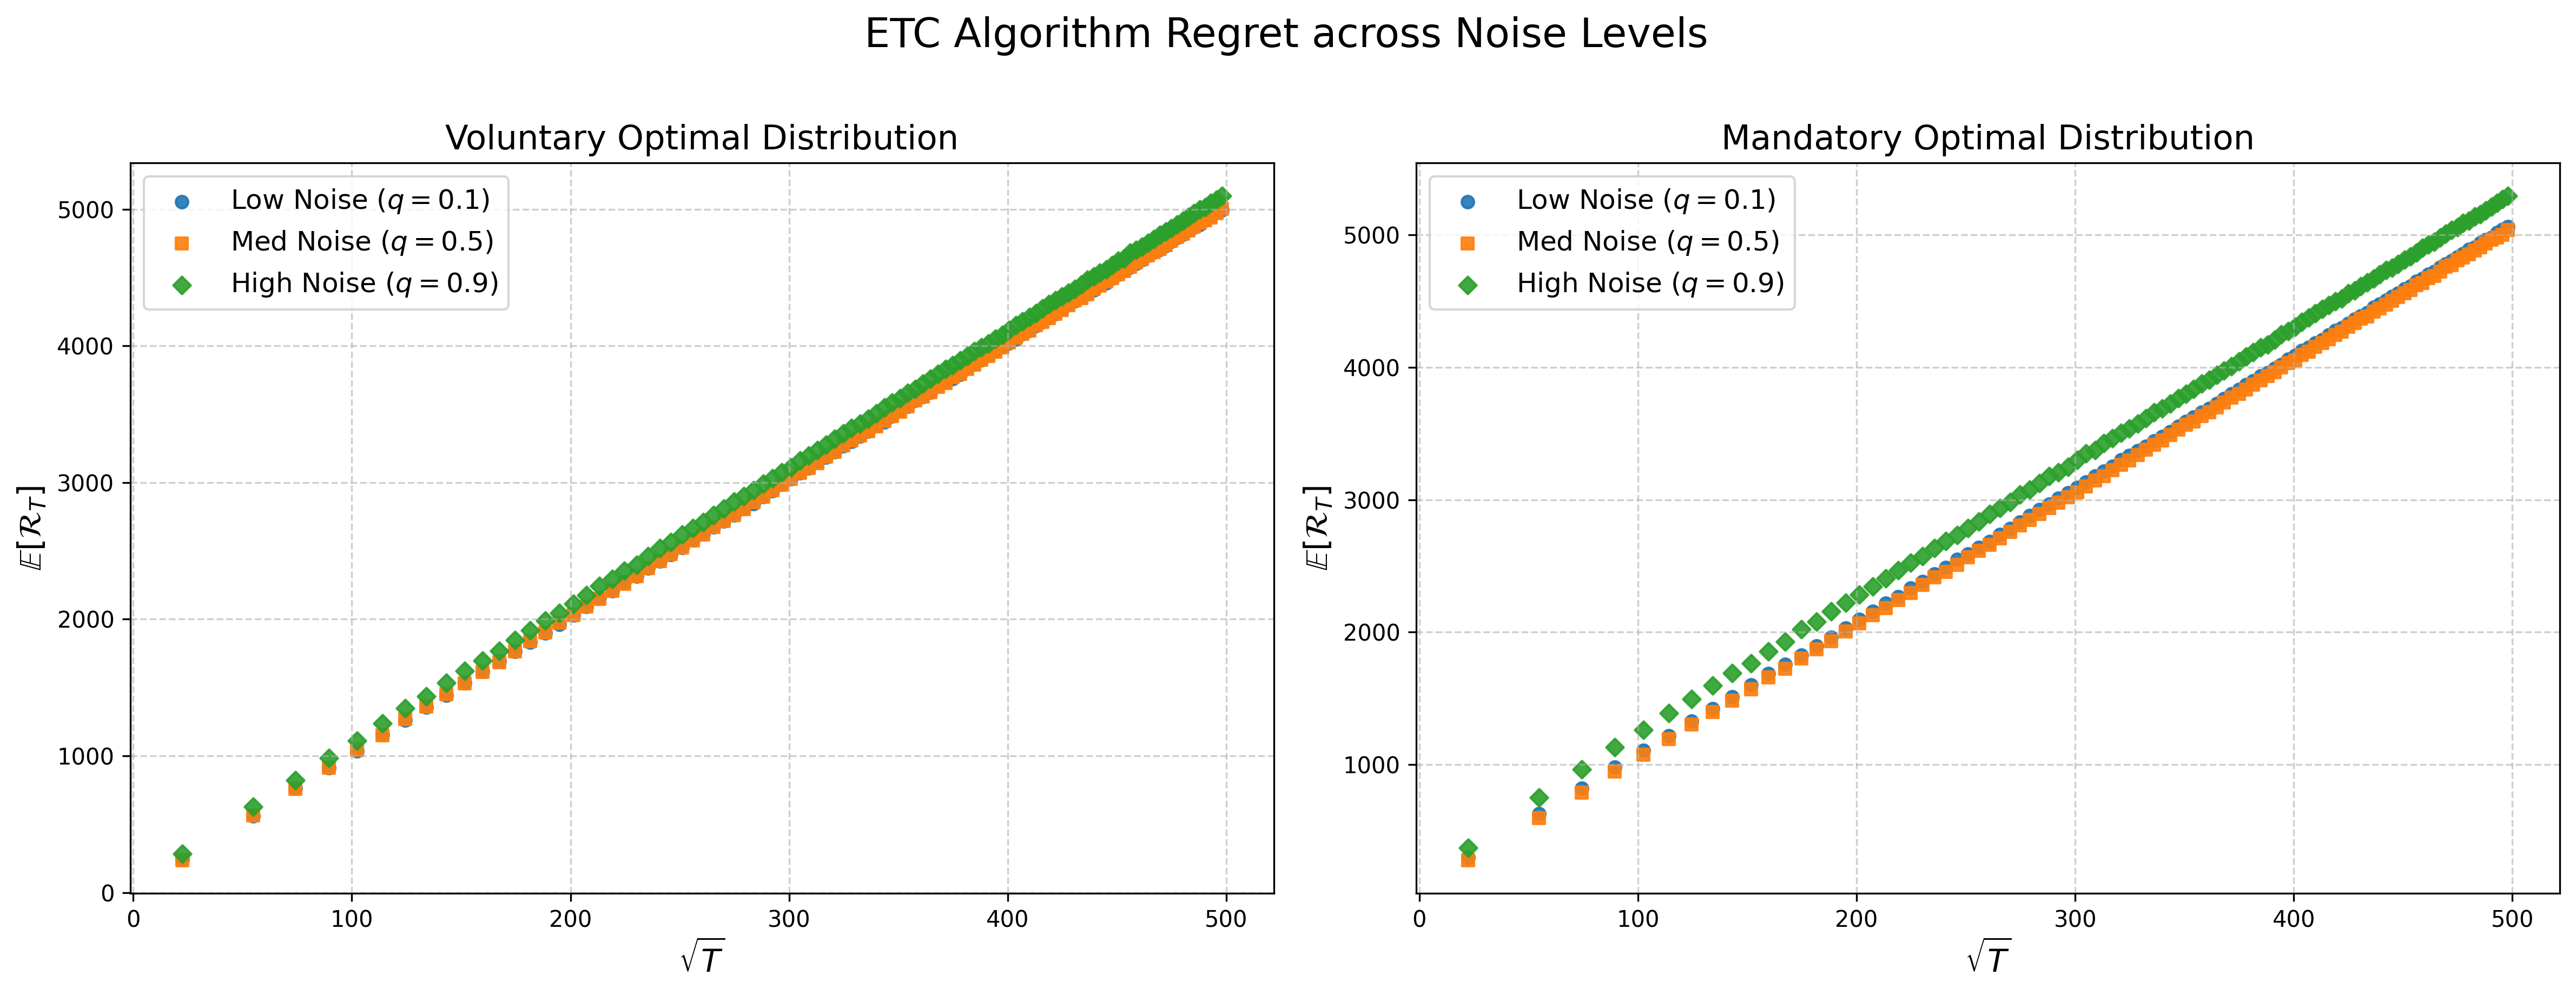
\includegraphics[height=0.5\textheight,width=0.85\textwidth,keepaspectratio]{dynamic_learning_regret.png}
        \end{figure}
    \end{columns}
\end{frame}

\section{Conclusion}

\begin{frame}{Conclusion}
    \begin{itemize}
        \item \textbf{Strategic Disclosures:} We modeled feature revelation as a game and showed that under certain quantifiable conditions, allowing participants to withhold features \textbf{improves} receiver's predictive accuracy.
        \item \textbf{Regression vs Classification:} Derived rigid "if and only if" bounds for Strategic Advantage, dependent on Sender-Receiver alignment $\Cov(U,Y)$.
        \item \textbf{Static and Dynamic Learning:} We showed that these concepts translate reliably to real-world learning problems where environment parameters must be deduced from samples or interactions, achieving $\mathcal{O}(\sqrt{T})$ dynamic regret limits.
    \end{itemize}
\end{frame}

\begin{frame}[allowframebreaks]{References}
    \nocite{*}
    \bibliography{references}
    \bibliographystyle{IEEEtran}
\end{frame}

\end{document}
